% !TEX root = ../main.tex

\section{Evaluating Proposed Solutions}\label{sec:eval}

In this section, we evaluate 10 solutions that have been proposed by Ethereum community---mostly from developers on GitHub---to address the multiple withdrawal attack. We examine each solution in detail and evaluate them against the criteria established in the previous section (see Section~\ref{sec:criteria}). The summary is presented in Table~\ref{tab:comp}.

\subsection{Enforcement by User Interface (UI)}
\label{sec:enfui}

\begin{figure}[t!]
	\centering
	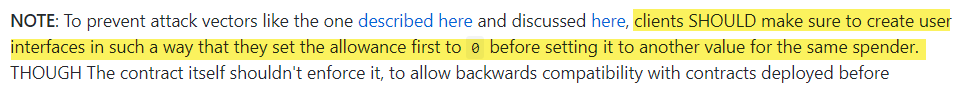
\includegraphics[width=1.0\linewidth]{figures/multiple_withdrawal_03.png}
	\caption{Recommendation of ERC20 standard to mitigate multiple withdrawal attack by enforcement in UI.\label{fig:uie}}
\end{figure}

The first solution is enforcement at the user interface level. We discussed this previously in Section~\label{sec:preui} but we reiterate the main points here again. The exact recommendation from the ERC20 standard is shown in Figure~\ref{fig:uie} and is essentially to set an allowance to zero before any non-zero values. Presumedly, it will also enforce that the new approval is not allowed if proceeded by a token transfer by the approved spender. We consider the UI to be a lightweight web app that can reference a contract's state variables and emitted events but does not maintain a full copy of the blockchain. Consider (again) the most basic attack sequence:

% Jeremy: Even with logging events, if Bob sends to Carol, then Alice won't necessarily pause before step 5

\begin{enumerate}
	\item Alice allows Bob to transfer N of Alice's tokens.
	\item Alice's client broadcasts an allowance of 0 for Bob.
	\item Bob broadcasts a competing transaction to transfer N of Alice’s tokens.
	\item Bob's transaction front-runs Alice's, is confirmed, and sets Bob’s allowance to 0 (from N).
	\item Alice’s transaction is confirmed and sets Bob’s allowance to 0 (from 0).
	\item Alice's client broadcasts an allowance of M for Bob.
	\item Alice’s second transaction is confirmed and sets Bob's allowance to M.
	\item Bob transfers M of Alice’s tokens for a total of N+M tokens.
\end{enumerate}

The key mitigation to this attack is for Alice's client to pause at step 6 and determine if a transaction sequence like 3\&4 has occurred or not. This cannot be determined by monitoring the integer that records Bob's allowance because it will be 0 regardless of whether 3\&4 occurred or not. It also cannot always be determined by monitoring the events omitted from the contract. Step 4 will log a transfer from Alice's address to Bob's address of N tokens. If no event is omitted, Alice can know for certain no transfer was made. However if an event is emitted, Alice must decide it was a transfer initiated by Bob or a transfer by someone else she has authorized. If she has not authorized anyone else, she can know for certain it was Bob. However if she has a busy account with multiple authorized spenders of her tokens, the event is not verbose enough to determine what happened. Importantly, it does not record who initiated the transfer, only who received the tokens, and these are not necessarily the same entity. Bob can send Alice's tokens to his accomplice Carol, or some other authorized spender can send Alice's tokens to Bob (which looks like Bob is attacking when he is not). Since a UI is automated and does not use human discretion, it cannot decide circumstantially whether something looks like an attack or not --- it must either specify exact rules which it cannot do precisely for ambiguous events or it can ask for Alice's human input which introduces usability issues. In conclusion, it is better for enforcement to happen at the contract level. The trick for approving 0 and then approving N can be implemented. 

\textblue{Expand on this.} Interestingly, OpenZeppelin example implements a workaround in contract level but the added parameters make it inconsistent with the standard UI recommendations.



\subsection{Minimum viable token}
As suggested by Ethereum Foundation\cite{Ref05}, we can boil down ERC20 standard to a very basic functionalities by implementing only essential methods. This prevents effecting of the attack by skipping implementation of vulnerable functions. While removing \texttt{approve} and \texttt{transferFrom} functions prevent the attack, it makes the token partially-ERC20-compliant. Golem Network Token (GNT\footnote{https://etherscan.io/address/0xa74476443119A942dE498590Fe1f2454d7\newline D4aC0d\#code}) is one of these examples since it does not implement the \texttt{approve}, \texttt{allowance} and \texttt{transferFrom} functions. According to ERC20 specifications\cite{Ref08}, these methods are not OPTIONAL and must be implemented. Moreover, ignoring them will cause failed function calls from standard smart contracts that expect to interoperate with these methods. Therefore, we would not consider it as a backward compatible solution although mitigates the attack.

\subsection{Approving trusted parties}
Approving token transfer to parties that we trust, reduces risk of impacting by the attack. Non-upgradable smart contracts or trusted accounts can be considered safe for delegating token transfers on behalf of us. Because they do not contain any logic to take advantage of this vulnerability. However, upgradable smart contracts may add new code to their new versions that needs code re-verification before approving token transfers. Similarly, approving token transfer to people that we trust could be considered as a mitigation plan. Nonetheless, this solution would have limited use cases and it could not be considered as a universal preventive approach.

\begin{figure}[t]
	\centering
	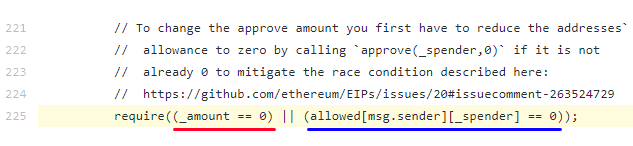
\includegraphics[width=1.0\linewidth]{figures/multiple_withdrawal_06.png}
	\caption{MiniMeToken added code to \texttt{approve} method for allowing non-zero allowance values if it is already set to zero.\label{fig:mini}}
\end{figure}
\begin{comment}
// To change the approve amount you first have to reduce the addresses`
//  allowance to zero by calling `approve(_spender,0)` if it is not
//  already 0 to mitigate the race condition described here:
//  https://github.com/ethereum/EIPs/issues/20#issuecomment-263524729
require((_amount == 0) || (allowed[msg.sender][_spender] == 0));
\end{comment}
\subsection{MiniMeToken}\label{sec:MiniMeToken}
MiniMeToken\cite{Ref15} follows ERC20 recommendation for setting allowance to zero before non-zero values. Token holder needs to execute two transactions, setting allowance from N to zero and then from 0 to M. MiniMeToken added a new line of code to the \texttt{approve} method for preventing the attack by enforcing this rule (see Figure~\ref{fig:mini}). The red clause in line 225 (\texttt{\_amount == 0}) allows setting of approval to 0 and blue condition checks allowance of \texttt{\_spender} to be 0 before setting to non-zero values (\ie If \texttt{\_spender} allowance is 0 then allows non-zero values). Similar to~\ref{sec:enfui}, this solution will not prevent Bob from transferring N+M tokens. Because Alice would not be able to distinguish whether N tokens have been already drained by Bob or not. Considering the below scenario:
\begin{enumerate}
	\item Alice decides to set Bob’s allowance to 0.
	\item Bob front-runs Alice’s transaction and his allowance sets to 0 after transferring N tokens.
	\item Alice’s transaction is executed and sets Bob’s allowance to 0 (Red clause passes sanity check).
	\item Alice checks Bob’s allowance and she will find it 0, so, she can not determine whether this was because of her transaction or Bob already transferred N tokens.
	\item Alice considers that Bob has not transferred any tokens and allows him for transferring new M tokens.
	\item Bob is able to transfer new M tokens and N+M in total.
\end{enumerate}


% Jeremy: We require it to be zero but don't know if it is zero because it was reset or because it was drained

\begin{figure}[t]
	\centering
	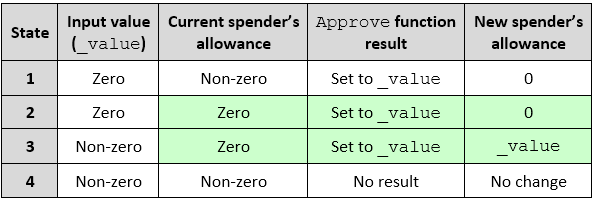
\includegraphics[width=1.0\linewidth]{figures/multiple_withdrawal_09.png}
	\caption{Functionality of default \texttt{approve} method in MonolithDAO token that enforces setting spender's allowance to zero before any non-zero values. It implements ERC20 recommendation for changes allowance from N to M in two steps (N$\rightarrow$0$\rightarrow$M).\label{fig:dao}}
\end{figure}

\subsection{MonolithDAO}
MonolithDAO Token\cite{Ref12} implements two additional functions for allowance increase\footnote{\texttt{increaseApproval(address \_spender, uint \_addedValue)}} or decrease\footnote{\texttt{decreaseApproval(address \_spender, uint \_subtractedValue)}}. The default \texttt{approve} function has additional codes to enforce the owner for setting allowance to zero before non-zero values. It allows non-zero spender's allowance if it is already set to zero (see Figure~\ref{fig:dao}). If the current spender’s allowance is non-zero, \texttt{decreaseApproval} and \texttt{increaseApproval} functions have to be used instead of standard \texttt{approve} method as explained below:
\begin{enumerate}
	\item Alice allows Bob to transfer N tokens by calling \texttt{approve(\_Bob, N)}. Alice used the default \texttt{approve} function consciously since current Bob’s allowance is 0. So, he checked Bob's allowance before calling \texttt{approve} method.
	\item After a while, Alice decides to decrease Bob’s approval by M and runs \texttt{decreaseApproval(\_Bob, M)}.
	\item Bob notices Alice’s second transaction and front runs it by executing \texttt{transferFrom(\_Alice, \_Bob, N)}.
	\item Bob’s transaction will be executed first and transfers N token to his account and the his allowance becomes 0 as result of this transfer.
	\item Alice’s transaction is mined after Bob’s transaction and tries to decrease Bob’s allowance by M. If Bob had already transferred more than M tokens, new Bob’s allowance becomes negative and it fails the transaction. So, the transaction does not change Bob’s remaining allowance and he would be able to transfer the rest (which is legitimate transfer since Alice has already approved it). If Bob had transferred less than M tokens, the new allowance will be applied and reduces Bob’s allowance by M.
\end{enumerate}
\noindent Although these two new complementary functions prevent the attack, they have not been defined in the initial specifications of ERC20 standard. Therefore, they can not be used by smart contracts that are already deployed on the Ethereum network and still call \texttt{approve} method for setting new allowance---and not \texttt{increaseApproval} or \texttt{decreaseApproval}. Moreover, ERC20 specifications does not define any increase or decrease of allowance. It only allows setting new allowances without adjustment. For example, if Alice has approved Bob for 100 tokens and wants to set it to 80, the new allowance should be 80 while using decrease methods will set it to 20 (100 - 80 = 20). Comparatively, increase method sets new allowance to 180 while it has to set it to 80 again to be in-compliant with ERC20 specification. For these reasons, this solution would not be compatible with ERC20 standard and only is usable if approver or smart contract are aware of these supplementary methods.


\subsection{Alternate approval function}
Another suggestion\cite{Ref16} is to move security checks to another function called \texttt{safeApprove}\footnote{\texttt{safeApprove(address \_spender, uint256 \_currentValue, uint256 \_value}} that compare current and new allowance value and sets it if has not been already changed. By using this function, Alice uses the standard \texttt{approve} function to set Bob’s allowance to 0 and for new approvals, she has to use \texttt{safeApprove} function. \texttt{safeApprove} takes the current expected approval amount as input parameter and calls \texttt{approve} method if previous allowance is equal to the current expected approval. By using this function, Alice will have one step more to read the current allowance and pass it to the new \texttt{safeApprove} method. Although this approach mitigates the attack by using CAS pattern\cite{Ref06}, however, it is not backward compatible with already implemented smart contracts due to their unawareness of this new complementary function. In other words, the new \texttt{safeApprove} method is not defined in ERC20 standard and existing smart contracts would not be able to use this new safety feature.

\subsection{Detecting token transfers}
In order to set new allowance atomically, tracking of transferred tokens is required to detect token transfers before setting new allowances. If \texttt{approve} method reveals any transferred tokens due to front running, it throws an exception without setting new allowance. As suggested by \cite{Ref17}, a flag can be used to detect whether any token has been transferred or not. \texttt{transferFrom} method sets this flag to \texttt{true} in case of any token transfer. \texttt{approve} method checks the flag to be \texttt{false} before allowing new approvals. This approach requires new data structure to keep track of used/transferred tokens for each spender. It can prevent front-running in the below scenario:
\begin{enumerate}
	\item Alice runs \texttt{approve(\_Bob, N)} to allow Bob for transferring N tokens. Since Bob’s initial allowance is 0 and his corresponding flag=\texttt{false}, then sanity check passes and Bob’s allowance sets to N (line 16).
	\item Alice decides to set Bob’s allowance to 0 by executing \texttt{approve(\_Bob, 0)}.
	\item Bob front-runs Alice’s transaction and transfers N tokens. Then, \texttt{transferFrom} turns his flag to \texttt{true}.
	\item Alice’s transaction is mined and passes sanity check because passed value is 0 in line 15.
	\item Bob’s allowance is set to 0 while his flag remains \texttt{true}. (\texttt{approve} method does not flip spender flags.)
	\item Alice wants to change Bob’s allowance to M by executing \texttt{approve(\_Bob, M)}. Since Bob already transferred N tokens (his flag=\texttt{true}), then transaction fails.
	\item Bob’s allowance does not change and he cannot move more tokens than initially allowed.
\end{enumerate}
\noindent Although this approach mitigates the attack, but it prevents any further legitimate approvals as well. Considering a scenario that Alice rightfully wants to increase Bob’s allowance from N to M (two non-zero values). If Bob had already transferred number of tokens, Alice would not be able to change his approval. Because Bob's flag is set to \texttt{true} and line 15 does not allow changing allowance by throwing an exception (see Figure~\ref{fig:det}).
\begin{figure}[t]
	\centering
	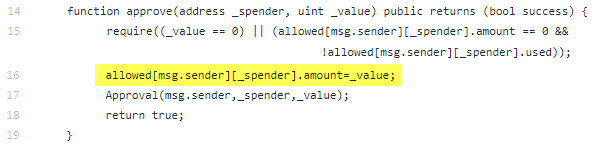
\includegraphics[width=1.0\linewidth]{figures/multiple_withdrawal_33.png}
	\caption{\texttt{approve} method needs to be modified by adding a line of code like \texttt{allowed[msg.sender][\_spender].used = false;} between lines 16 and 17 to unlock spender flag for the next legitimate change. However, this change makes attack mitigation ineffective.\label{fig:det}}
\end{figure}
\begin{comment}
function approve(address _spender, uint _value) public returns (bool success) {
	require((_value == 0) || (allowed[msg.sender][_spender].amount == 0 && !allowed[msg.sender][_spender].used));
	allowed[msg.sender][_spender].amount=_value;
	Approval(msg.sender,_spender,_value);
	return true;
}
\end{comment}
\noindent Even setting allowance to 0 and then to M, does not flip the flag to \texttt{false} (There is no code for it in the \texttt{approve} method). So, It keeps Bob’s allowance locked down and blocked further legitimate allowances. In fact, \texttt{approve} method needs a new code between lines 16 and 17 to set the flag to \texttt{false}. But it will cause another problem. After setting allowance to 0, spender flag becomes \texttt{false} and allows non-zero values even if tokens have been already transferred. Considering front-running by Bob in the below scenario:
\begin{enumerate}
	\item Alice changes Bob's allowance from N to 0.
	\item Bob transfers N tokens before allowance change and his \texttt{used} flag turns to \texttt{true}.
	\item Alice's transaction is successful since \texttt{\_value=0}. (The second condition is not evaluated although \texttt{used} flag is \texttt{true}).
	\item Alice transaction turns \texttt{used} flag to \texttt{false} and sets Bob's allowance to 0. 
	\item Now Alice wants to set Bob's allowance from 0 to M, His flag is \texttt{false} and allowance is 0. So, Alice cannot distinguish whether Bob moved any token or not. Setting new allowance will allow Bob to transfer more tokens than Alice wanted.
\end{enumerate}
In fact, resetting the flag in \texttt{approve} method will not fix the issue and makes attack mitigation ineffective. In short, this approach can not satisfy both legitimate and non-legitimate scenarios. Nevertheless, it is a step forward by introducing the need for a new variable to track transferred tokens.\newline

\subsection{Keeping track of remaining tokens}
This approach\cite{Ref18} is inspired by the previous solution and keeping track of remaining tokens instead of detecting transferred tokens. \texttt{approve} method uses these variables to set allowance accordingly. It uses modified version of data structure that used in the previous solution for storing residual tokens (see Figure~\ref{fig:track}).
\begin{figure}[t]
	\centering
	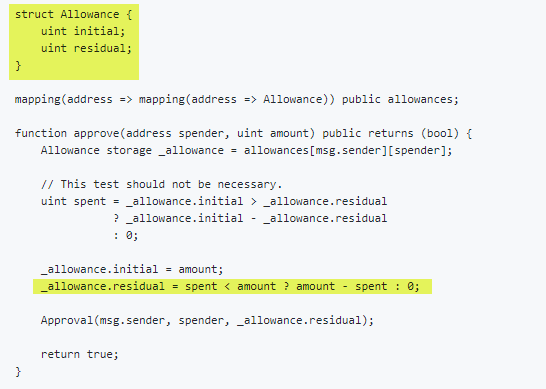
\includegraphics[width=1.0\linewidth]{figures/multiple_withdrawal_29.png}
	\caption{Keeping track of remaining tokens by introducing new data structure.\label{fig:track}}
\end{figure}
\begin{comment}
struct Allowance {
	uint initial;
	uint residual;
}

mapping(address => mapping(address => Allowance)) public allowances;

function approve(address spender, uint amount) public returns (bool) {
	Allowance storage _allowance = allowances[msg.sender][spender];
	
	// This test should not be necessary.
	uint spent = _allowance.initial > _allowance.residual
	? _allowance.initial - _allowance.residual
	: 0;
	
	_allowance.initial = amount;
	_allowance.residual = spent < amount ? amount - spent : 0;
	
	Approval(msg.sender, spender, _allowance.residual);
	
	return true;
}

function allowance(address holder, address spender) public view returns (uint) {
	return allowances[holder][spender].residual;
}

function transferFrom(address holder, uint amount) public returns (bool) {
	uint residual = allowance(holder, msg.sender);
	
	require(amount <= residual);
	
	allowances[holder][msg.sender].residual = residual - amount;
	
	// ... do the token transfer
	
	return true;
}
\end{comment}
\noindent At the first look, it seems to be a promising solution by setting approval to zero before non-zero values. However, the highlighted code in \texttt{approve} method resembles the situation that is explained in~\ref{sec:enfui}. In case of front-running, both \texttt{initial} and \texttt{residual} variables will be zero and it would not be possible for Alice to distinguish if any token transfer have occurred due to her allowance change or Bob token transfer. To make it more clear, considering the below scenario:  
\begin{enumerate}
	\item Bob’s allowance is initially zero (\texttt{allowances[\_Alice][\_Bob].initial=0}) and his residual is zero as well (\texttt{allowances[\_Alice][\_Bob].residual=0}).
	\item Alice allows Bob to transfer N tokens that makes \texttt{allowances[\_Alice][\_Bob].initial=N} and \texttt{allowances[\_Alice][\_Bob].residual=N}.
	\item Alice decides to change Bob’s allowance to M and has to set it to zero before any non-zero.
	\item Bob noticed Alice’s transaction for setting his allowance to zero and transfers N tokens in advance. Consequently, \texttt{transferFrom} function sets his residual to zero (\texttt{allowances[\_Alice][\_Bob].residual=0}).
	\item Alice’s transaction for setting Bob's allowance to zero is mined and sets \texttt{allowances[\_Alice][\_Bob].initial=0} and \texttt{allowances[\_Alice][\_Bob].residual=0} This is similar to step 1 that no token has been transferred. So, Alice would not be able to distinguish whether any token have been transferred or not.
	\item Considering no token transfer by Bob, Alice approves Bob for spending new M tokens.
	\item Bob is able to transfer new M tokes in addition to initial N tokens.\newline
\end{enumerate}
Someone may think of using \texttt{Transfer} event to detect transferred tokens or checking approver balance to see any transferred tokens. As explained in~\ref{sec:enfui}, using \texttt{Transfer} event is not sufficient in case of transferring tokens to a third party. Checking approver balance also would not be an accurate way if the contract is busy and there are lot of transfers. So, it would be difficult for the approver to detect legitimate from non-legitimate tokens transfers. Overall, this approach cannot prevent the attack.

\subsection{Changing ERC20 API}
As advised by \cite{Ref03}, changing ERC20 API could secure \texttt{approve} method by comparing current allowance of the spender and sets it to new value if he has not already been transferred any tokens. This allows atomic compare and set of spender allowance to make the attack impossible. This approach needs a new overloaded \texttt{approve} method with three parameters in addition to the standard \texttt{approve} method with two parameters (see Figure~\ref{fig:api}).

In order to use this new method, smart contracts have to update their codes to provide three parameters instead of current two, otherwise any \texttt{approve} call will use the standard vulnerable version with two parameters. Moreover, one more call is required to read current allowance and pass it to the new \texttt{approve} method. Additionally, new event definition needs to be added to ERC20 API to log an approval events with four arguments. For backward compatibility reasons, both three-arguments and new four-arguments events have to be logged. All of these changes makes this token contract incompatible with already deployed smart contracts. Hence, we would not consider it as a sustainable solution.
\begin{figure}[t]
	\centering
	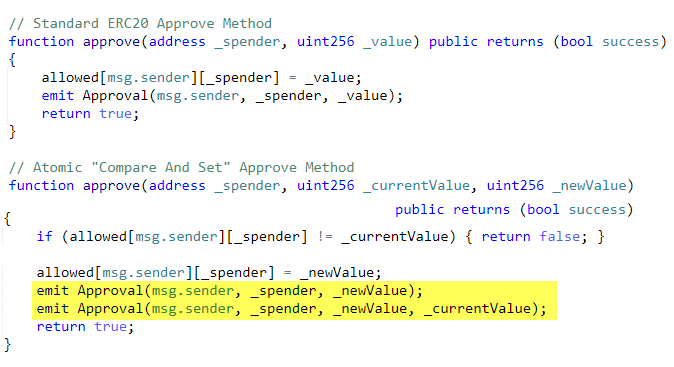
\includegraphics[width=1.0\linewidth]{figures/multiple_withdrawal_12.png}
	\caption{Suggested ERC20 API Change by adding new \texttt{approve} method with three parameters to compare and set new allowance atomically.\label{fig:api}}
\end{figure}
\begin{comment}
// Standard ERC20 Approve method
function approve(address _spender, uint256 _tokens) public returns (bool success) 
{

allowed[msg.sender][_spender] = _tokens;
emit Approval(msg.sender, _spender, _tokens);
return true;
}

// Atomic "Compare and Set" Approve method
function approve(address _spender, uint256 _currentValue, uint256 _newValue) returns (bool success)
{
if(allowed[msg.sender][_spender] != _currentValue) {return false};
allowed[msg.sender][_spender] = _newValue;
emit Approval(msg.sender, _spender, _newValue);
emit Approval(msg.sender, _spender, _newValue, _currentValue);
return true;
}
\end{comment}
\subsection{New token standards}
Most of the new token standards are introduced to improve current functionality of ERC20 tokens and do not address the attack (see Table~\ref{tab:erc}). Despite these enhancements, migration from ERC20 to new token standard would not be convenient and all deployed ERC20 tokens---168,092 tokens\footnote{https://etherscan.io/tokens, Accessed 18-Feb-2019}---have to be redeployed. This also means update of trading platform who already listed ERC20 tokens. Our goal is to find a backward compatible solution instead of changing current ERC20 API or migrating tokens to a new standards. Despite expanded features and improved security properties of new standards, we would not consider them as a target solutions.
\begin{table}
\centering
\begin{tabular}{|m{1.3cm}|m{6cm}|}
	\hline\centering
	Token Standard & A description of non-compliance with ERC20\\
	\hline\hline\centering
	ERC 223 \cite{Ref20} & It does not implement ERC20 \texttt{approve} + \texttt{transferFrom} mechanism by assuming it potentially insecure and inefficient.\\ 
	\hline\centering 
	ERC 667 \cite{Ref21} & It solves the problem of transfer function in ERC223 (i.e., The need to implement \texttt{onTokenTransfer} routing in the receiving contract). So, it does address the attack and uses the same code as ERC223 with a supplementary function.\\ 
	\hline\centering 
	ERC 721 \cite{Ref22} & Unlike ERC20 tokens that share the same characteristics, ERC721 tokens represent a non-fungible tokens (NFT) which are unique and non-interchangeable with each other. In addition to this differences, ERC721 does not implement \texttt{transfer} method of ERC20 standard and introduces a safe transfer function defined as \texttt{safeTransferFrom}.\\ 
	\hline\centering
	ERC 777 \cite{Ref23} & This standard does not use \texttt{transfer} and \texttt{transferFrom} methods of ERC20 and implements \texttt{send} and \texttt{operatorSend} instead. Moreover, costly \texttt{approve} + \texttt{transferFrom} mechanism is replaced by \texttt{tokensReceived} function. Therefore, it would not be backward compatible with ERC20 requirements. Nevertheless a token contract may implement both ERC20 and ERC777 in parallel which still requires attack mitigation.\\ 
	\hline\centering 
	ERC 827 \cite{Ref24} & It uses OpenZeppelin\cite{Ref10} ERC20 implementation and defines three new functions to allow users for transferring data in addition to value in ERC20 transactions. This feature enables ERC20 tokens to have the same functionality as Ether (transferring data and value). In fact, it extends functionality of ERC20 tokens and not addressing the attack. \\ 
	\hline\centering 
	ERC 1155 \cite{Ref25} & It is improved version of ERC721 by allowing each Token ID to represent a new configurable token type, which may have its own metadata, supply and other attributes. ERC1155 aimed to remove the need to "approve" individual token contracts separately. Therefore, it does not implement any code to address the vulnerability\\ 
	\hline\centering 
	ERC 1377 \cite{Ref26} & It implements \texttt{approve} method with three parameters in addition to the ERC20 default \texttt{approve} with two inputs. Additionally, it uses OpenZeppelin\cite{Ref10} approach for increasing and decreasing approvals. We would consider it as mix of MiniToken and OpenZeppelin approaches that we discussed before.\\
	\hline
\end{tabular}
\newline
\caption{Comparison of ERC standards in terms of com pliancy with ERC20 specification \label{tab:erc}}
\end{table}
